\documentclass[12pt,a4paper]{article}
% ===== Packages =====
\usepackage[utf8]{inputenc}
\usepackage[T1]{fontenc}
\usepackage{orcidlink}
\usepackage{authblk}
\usepackage[english]{babel}
\usepackage{amsmath, amssymb, amsthm}
\usepackage{mathtools}
\usepackage{algorithm}
\usepackage{algpseudocode}
\usepackage{booktabs}
\usepackage{hyperref}
\usepackage{geometry}
\usepackage{xcolor}
\usepackage{tcolorbox}
\usepackage{listings}
\usepackage{float}
\usepackage{tikz}
\usetikzlibrary{arrows.meta, positioning, calc, patterns, decorations.pathreplacing, shapes.geometric, matrix, backgrounds}
\tcbuselibrary{theorems, skins, breakable}
\geometry{margin=2.5cm}
% ===== Theorem Environments =====
\newtheorem{theorem}{Theorem}[section]
\newtheorem{lemma}[theorem]{Lemma}
\newtheorem{corollary}[theorem]{Corollary}
\newtheorem{definition}[theorem]{Definition}
\newtheorem{remark}[theorem]{Remark}
% ===== Color Boxes =====
\tcbset{
  keybox/.style={
    enhanced, breakable,
    colback=blue!5!white, colframe=blue!60!black,
    fonttitle=\bfseries, title=#1
  },
  warnbox/.style={
    enhanced, breakable,
    colback=orange!5!white, colframe=orange!70!black,
    fonttitle=\bfseries, title=#1
  },
  codebox/.style={
    enhanced, breakable,
    colback=gray!5!white, colframe=gray!60!black,
    fonttitle=\bfseries, title=#1
  }
}
% ===== Listings Style =====
\lstset{
  basicstyle=\ttfamily\small,
  keywordstyle=\color{blue}\bfseries,
  commentstyle=\color{gray},
  stringstyle=\color{red!70!black},
  numbers=left,
  numberstyle=\tiny\color{gray},
  numbersep=8pt,
  frame=single,
  breaklines=true,
  language=C++
}
% ===== Macros =====
\newcommand{\fl}{\mathrm{fl}}
\newcommand{\uu}{\mathbf{u}}
\newcommand{\RR}{\mathbb{R}}
\newcommand{\FF}{\mathbb{F}}
\newcommand{\NWP}{\mathtt{NWP}}
\newcommand{\Nc}{\mathtt{Nc}}
\newcommand{\Nd}{\mathtt{Nd}}
\newcommand{\Ns}{\mathtt{Ns}}
% ===== Title =====
\title{
  \LARGE \textbf{Theory and Implementation of Multi-Word Floating-Point Arithmetic} \\[0.5em]
  \large Derivations and Proofs for Double-Word / Triple-Word Arithmetic \\
  and Quasi Algorithms, with Application to Lattice QCD CGNE Solvers
}
\author[1]{Wei-Lun Chen \orcidlink{0000-0002-8542-9126}}
\affil[1]{Advancesoft, 17F West, Shin-Ochanomizu Bldg., 4-3, Kanda-Surugadai, Chiyoda-ku, Tokyo 101-0062, Japan \authorcr \textit{chen.weilun@advancesoft.jp}}
\date{\today}
% ==========================================================

\begin{document}
\maketitle
\tableofcontents
\newpage

% ##########################################################
% CHAPTER 1: MULTI-WORD ARITHMETIC
% ##########################################################

% ==========================================================
\section{Multi-Word Floating-Point Arithmetic}
\label{sec:multiword}

This chapter provides a self-contained derivation of Double-Word (DW) and
Triple-Word (TW) floating-point arithmetic and their Quasi variants (QDW,
QTW).
The motivation is the need for precision beyond IEEE 754 FP64 in
ill-conditioned linear systems, without resorting to software arbitrary-precision
libraries (e.g.\ MPFR) that are orders of magnitude slower.

% ----------------------------------------------------------
\subsection{Motivation and Historical Background}

The limits of FP64 precision were recognized long before GPU computing.
Key milestones in multi-word arithmetic include:

\begin{itemize}
  \item \textbf{M\o{}ller (1965)~\cite{Moller1965}:} introduced Quasi double-precision
        for floating-point addition---the earliest quasi algorithm.
  \item \textbf{Dekker (1971)~\cite{Dekker1971}:} formalized double-word arithmetic
        and the splitting technique for error-free multiplication.
  \item \textbf{Knuth (1969)~\cite{Knuth1969}:} proved the TwoSum algorithm for
        error-free addition.
  \item \textbf{Joldes, Muller, Popescu (2017)~\cite{Joldes2017}:} provided
        tight, rigorous error bounds for DW building blocks.
  \item \textbf{Fabiano, Muller, Picot (2019)~\cite{Fabiano2019}:} extended the
        analysis to Triple-Word arithmetic.
  \item \textbf{Mukunoki \& Ozaki (2025)~\cite{Mukunoki2025}:} demonstrated that
        Quasi variants suffice for iterative solvers when combined with one
        normalization per iteration---the key result motivating this work.
\end{itemize}

The central idea is illustrated in Figure~\ref{fig:multiword_concept}.

\begin{figure}[H]
\centering
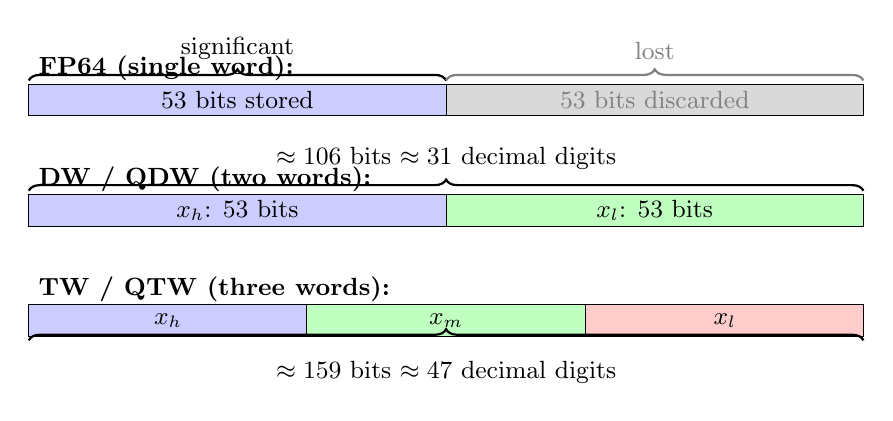
\begin{tikzpicture}[font=\small]
  % ---- FP64 single word ----
  \node[anchor=west] at (0, 2.8) {\textbf{FP64 (single word):}};
  \draw[fill=blue!20] (0,2.2) rectangle (5.3,2.6);
  \draw[fill=gray!30] (5.3,2.2) rectangle (10.6,2.6);
  \node at (2.65, 2.4) {53 bits stored};
  \node at (7.95, 2.4) {\color{gray}53 bits discarded};
  \draw[decorate, decoration={brace,amplitude=4pt}, thick]
    (0,2.65) -- (5.3,2.65) node[midway, above=4pt] {significant};
  \draw[decorate, decoration={brace,amplitude=4pt}, thick, color=gray]
    (5.3,2.65) -- (10.6,2.65) node[midway, above=4pt] {\color{gray}lost};
  % ---- DW / QDW ----
  \node[anchor=west] at (0, 1.4) {\textbf{DW / QDW (two words):}};
  \draw[fill=blue!20]  (0,  0.8) rectangle (5.3, 1.2);
  \draw[fill=green!25] (5.3,0.8) rectangle (10.6,1.2);
  \node at (2.65,1.0) {$x_h$: 53 bits};
  \node at (7.95,1.0) {$x_l$: 53 bits};
  \draw[decorate, decoration={brace,amplitude=4pt}, thick]
    (0,1.25) -- (10.6,1.25) node[midway, above=4pt] {$\approx 106$ bits $\approx 31$ decimal digits};
  % ---- TW / QTW ----
  \node[anchor=west] at (0, 0.0) {\textbf{TW / QTW (three words):}};
  \draw[fill=blue!20]  (0,   -0.6) rectangle (3.53, -0.2);
  \draw[fill=green!25] (3.53,-0.6) rectangle (7.07, -0.2);
  \draw[fill=red!20]   (7.07,-0.6) rectangle (10.6, -0.2);
  \node at (1.77,-0.4) {$x_h$};
  \node at (5.30,-0.4) {$x_m$};
  \node at (8.84,-0.4) {$x_l$};
  \draw[decorate, decoration={brace,amplitude=4pt}, thick]
    (0,-0.65) -- (10.6,-0.65) node[midway, below=4pt] {$\approx 159$ bits $\approx 47$ decimal digits};
\end{tikzpicture}
\caption{Conceptual layout of multi-word numbers. Each box is one FP64 word (53 bits).
DW/QDW doubles effective precision by retaining the discarded bits in $x_l$.
TW/QTW adds a third word $x_m$. The non-overlapping condition $|x_l|\leq\mathbf{u}|x_h|$
ensures the words tile the bit-line without gap or overlap.}
\label{fig:multiword_concept}
\end{figure}

\begin{tcolorbox}[keybox={The Fundamental Limitation of FP64}]
An FP64 significand has 52 explicit bits (53 with the implicit leading 1).
The exact product $a \times b$ may require up to \textbf{106 bits} to represent,
but FP64 truncates this to 53 bits.
The core idea of multi-word arithmetic is to \textbf{recover the discarded bits}
by storing them in additional floating-point words.

\medskip
Precision levels achievable with standard FP64 arithmetic:
\[
  \underbrace{\text{FP64} \times 1}_{\approx 16\;\text{digits}}
  \;\longrightarrow\;
  \underbrace{\text{DW/QDW} \times 2}_{\approx 31\;\text{digits}}
  \;\longrightarrow\;
  \underbrace{\text{TW/QTW} \times 3}_{\approx 47\;\text{digits}}
\]
\end{tcolorbox}

% ----------------------------------------------------------
\subsection{Floating-Point Notation and Prerequisites}
\label{sec:notation}

\begin{definition}[IEEE 754 Rounding Model]
Let $\FF$ denote the set of IEEE 754 double-precision (FP64) floating-point numbers.
For any real $x \in \RR$, the rounded value $\fl(x) \in \FF$ satisfies
\begin{equation}
  \fl(x) = x(1 + \delta), \qquad |\delta| \leq \uu,
  \label{eq:rounding_model}
\end{equation}
where $\uu = 2^{-53}$ is the \textbf{unit roundoff} (half the machine epsilon).
Equivalently, in additive error form:
\begin{equation}
  \fl(x) = x + \varepsilon, \qquad |\varepsilon| \leq \uu\,|x|.
\end{equation}
\end{definition}

\begin{definition}[Fused Multiply-Add (FMA)]
The FMA operation is defined as
\begin{equation}
  \mathrm{fma}(a, b, c) = \fl(ab + c).
\end{equation}
\textbf{Key property:} the product $ab$ is computed internally with full 106-bit
precision; only one rounding occurs at the very end.
This contrasts with the na\"{i}ve $\fl(\fl(a \cdot b) + c)$, which incurs
\emph{two} rounding steps.
FMA is available natively on all modern CPUs and GPUs (NVIDIA: \texttt{\_\_fma\_rn}).
\end{definition}

% ----------------------------------------------------------
\subsection{Basic Building Blocks: TwoSum and TwoProd}

\subsubsection{TwoSum: Error-Free Addition}

\begin{theorem}[TwoSum~\cite{Knuth1969,Moller1965}]
\label{thm:twosum}
Given $a, b \in \FF$, the following algorithm outputs $s = \fl(a + b)$ and
$e \in \FF$ satisfying
\begin{equation}
  a + b = s + e \quad \text{(exact, with no rounding error)}.
  \label{eq:twosum_exact}
\end{equation}

\begin{algorithm}[H]
\caption{$\mathrm{TwoSum}(a, b) \to (s,\, e)$}
\begin{algorithmic}[1]
\State $s \leftarrow \fl(a + b)$
\State $v \leftarrow \fl(s - a)$
\State $e \leftarrow \fl\bigl((a - \fl(s - v)) + (b - v)\bigr)$
\State \Return $(s,\; e)$
\end{algorithmic}
\end{algorithm}
\end{theorem}

\begin{proof}
\textbf{Step 1.}
Let $\varepsilon_s$ be the rounding error of the addition:
\begin{equation}
  s = (a + b) - \varepsilon_s, \qquad |\varepsilon_s| \leq \uu\,|a + b|.
\end{equation}

\textbf{Step 2.}
Compute $v = \fl(s - a)$.
Since $s \approx a + b$, we have $s - a \approx b$, so $v$ approximates
``the contribution of $b$ contained in $s$''.

\textbf{Step 3.}
Decompose the total error:
\begin{align}
  \delta_a &:= a - \fl(s - v)
    & &\text{(the part of $a$ ``lost'' in the sum)}, \\
  \delta_b &:= b - v
    & &\text{(the part of $b$ ``lost'' in the sum)}.
\end{align}
Then $e = \delta_a + \delta_b$.
One can show from IEEE 754 properties that $|\delta_a|, |\delta_b| \leq \uu\,|s|$,
so their sum is exactly representable:
$\fl(\delta_a + \delta_b) = \delta_a + \delta_b$.

Hence $a + b = s + e$ holds exactly. \qquad $\checkmark$
\end{proof}

\begin{remark}
Equation~\eqref{eq:twosum_exact} is an \textbf{exact identity} under IEEE 754
arithmetic, not an approximation.
It forms the cornerstone of all multi-word arithmetic.
\end{remark}

\subsubsection{TwoProd: Error-Free Multiplication}

\begin{theorem}[TwoProd via FMA~\cite{Dekker1971}]
\label{thm:twoprod}
Given $a, b \in \FF$, define
\begin{align}
  p &:= \fl(a \times b), \\
  e &:= \mathrm{fma}(a,\, b,\, -p).
\end{align}
Then
\begin{equation}
  ab = p + e \quad \text{(exact)}.
  \label{eq:twoprod_exact}
\end{equation}
\end{theorem}

\begin{proof}
By definition of FMA:
$e = \mathrm{fma}(a, b, -p) = \fl(ab - p)$.
The rounding error $ab - p = ab - \fl(ab)$ is at most $\uu|ab|$ in magnitude,
which is exactly representable in FP64 (Sterbenz-like argument).
Hence $\fl(ab - p) = ab - p$, giving $p + e = ab$ exactly. \qquad $\checkmark$
\end{proof}

\begin{tcolorbox}[warnbox={Without FMA: Dekker Splitting}]
When FMA is unavailable, use Dekker splitting with $\sigma = 2^{27} + 1$
to split $a = a_h + a_l$ (each 26 bits):
\[
  c = \fl(\sigma \cdot a), \quad
  a_h = \fl(c - (c - a)), \quad
  a_l = a - a_h,
\]
and similarly for $b$.
This requires \textbf{17 flops} versus \textbf{2} with FMA.
On modern CPUs and NVIDIA GPUs, always prefer the FMA-based TwoProd.
\end{tcolorbox}

% ----------------------------------------------------------
\subsection{Double-Word (DW) Arithmetic}
\label{sec:dw}

\subsubsection{Definition}

\begin{definition}[Double-Word Number]
A pair $(x_h, x_l) \in \FF^2$ satisfying the \textbf{non-overlapping condition}
\begin{equation}
  |x_l| \leq \uu\,|x_h|
  \label{eq:nonoverlap_dw}
\end{equation}
is called a \textbf{Double-Word (DW) number} representing the value
$x := x_h + x_l$.

The condition~\eqref{eq:nonoverlap_dw} ensures that the significand bits of
$x_h$ and $x_l$ do not overlap: $x_l$ extends $x_h$ in the lower bits,
yielding an effective precision of $2 \times 53 = 106$ bits.
\end{definition}

\begin{remark}
Bit-level picture of a DW number:
\begin{center}
\begin{tabular}{|c|c|}
\hline
$x_h$ significand (53 bits) & $x_l$ significand (next 53 bits) \\
\hline
\end{tabular}
\end{center}
$x_l$ continues the precision of $x_h$ into the lower-order bits.
\end{remark}

\subsubsection{DW Addition}

\begin{theorem}[DWadd~\cite{Joldes2017}]
Let $x = x_h + x_l$ and $y = y_h + y_l$ be DW numbers.
The following algorithm computes a DW number $z = z_h + z_l$ with
$|x + y - (z_h + z_l)| \leq O(\uu^2\,|x + y|)$.

\begin{algorithm}[H]
\caption{$\mathrm{DWadd}(x_h, x_l,\; y_h, y_l) \to (z_h,\, z_l)$}
\begin{algorithmic}[1]
\State $(s,\; e_1) \leftarrow \mathrm{TwoSum}(x_h,\; y_h)$
  \Comment{Error-free addition of high words}
\State $e_2 \leftarrow \fl(x_l + y_l)$
  \Comment{Approximate sum of low words}
\State $e_3 \leftarrow \fl(e_1 + e_2)$
  \Comment{Aggregate errors}
\State $(z_h,\; z_l) \leftarrow \mathrm{TwoSum}(s,\; e_3)$
  \Comment{\textbf{Normalization step}}
\State \Return $(z_h,\; z_l)$
\end{algorithmic}
\end{algorithm}
\end{theorem}

\begin{proof}
\textbf{Step 1.}
By Theorem~\ref{thm:twosum}: $s + e_1 = x_h + y_h$ (exact), $|e_1| \leq \uu\,|s|$.

\textbf{Step 2.}
$e_2 = x_l + y_l + \varepsilon_2$, $|\varepsilon_2| \leq \uu\,|x_l + y_l|$.
By non-overlapping, $|x_l|, |y_l| \leq \uu\,|x_h|$, so $|\varepsilon_2| \leq 2\uu^2\,|x_h|$ (second-order).

\textbf{Step 3.}
Accumulating: $x + y = s + e_3 + O(\uu^2\,|x_h|)$.

\textbf{Step 4 (Normalization).}
The final TwoSum$(s, e_3) \to (z_h, z_l)$ restores the non-overlapping condition:
$z_h + z_l = s + e_3$ (exact), $|z_l| \leq \uu\,|z_h|$. \qquad $\checkmark$
\end{proof}

\subsubsection{Quasi DW Addition (QDWadd)}

\begin{definition}[QDWadd]
\textbf{QDWadd} is obtained from DWadd by \emph{omitting the final normalization}
(line 4 of DWadd):

\begin{algorithm}[H]
\caption{$\mathrm{QDWadd}(x_h, x_l,\; y_h, y_l) \to (z_h,\, z_l)$}
\begin{algorithmic}[1]
\State $(s,\; e_1) \leftarrow \mathrm{TwoSum}(x_h,\; y_h)$
\State $e_2 \leftarrow \fl(x_l + y_l)$
\State $e_3 \leftarrow \fl(e_1 + e_2)$
\State $z_h \leftarrow s$;\quad $z_l \leftarrow e_3$
  \Comment{{\color{red}Final TwoSum omitted}}
\State \Return $(z_h,\; z_l)$
\end{algorithmic}
\end{algorithm}
\end{definition}

\begin{remark}[Cost and consequence of Quasi]
Without the final TwoSum, the non-overlapping condition may be \emph{violated}.
If QDWadd is applied repeatedly without repair, $z_l$ can grow and erode the
precision of $z_h$---called \textbf{drift} (see Section~\ref{sec:drift}).

\begin{center}
\begin{tabular}{lcc}
\toprule
 & \textbf{DWadd} & \textbf{QDWadd} \\
\midrule
Accuracy (single call)    & $O(\uu^2)$  & $O(\uu^2)$ \\
Non-overlapping guaranteed & Yes        & No         \\
Floating-point operations  & 12         & 6          \\
Stability under iteration  & Stable     & Drifts (needs repair) \\
\bottomrule
\end{tabular}
\end{center}
\end{remark}

\subsubsection{DW Multiplication}

\begin{theorem}[DWmul~\cite{Joldes2017}]
Let $x = x_h + x_l$ and $y = y_h + y_l$ be DW numbers.
The exact product expands as
\begin{equation}
  xy = \underbrace{x_h y_h}_{O(1)}
     + \underbrace{x_h y_l + x_l y_h}_{O(\uu)}
     + \underbrace{x_l y_l}_{O(\uu^2),\;\text{negligible}}.
\end{equation}

\begin{algorithm}[H]
\caption{$\mathrm{DWmul}(x_h, x_l,\; y_h, y_l) \to (z_h,\, z_l)$}
\begin{algorithmic}[1]
\State $(p,\; e_1) \leftarrow \mathrm{TwoProd}(x_h,\; y_h)$
  \Comment{Leading term (exact)}
\State $e_2 \leftarrow \fl(x_h \cdot y_l)$;\quad $e_3 \leftarrow \fl(x_l \cdot y_h)$
\State $(e_4,\; e_5) \leftarrow \mathrm{TwoSum}(e_2,\; e_3)$
\State $(e_6,\; e_7) \leftarrow \mathrm{TwoSum}(e_1,\; e_4)$
\State $e_8 \leftarrow \fl(e_5 + e_7)$
\State $(z_h,\; z_l) \leftarrow \mathrm{TwoSum}(p,\; e_6)$
\State $z_l \leftarrow \fl(z_l + e_8)$
\State \Return $(z_h,\; z_l)$
\end{algorithmic}
\end{algorithm}
\end{theorem}

\begin{definition}[QDWmul]
QDWmul omits the final TwoSum normalization of DWmul:

\begin{algorithm}[H]
\caption{$\mathrm{QDWmul}(x_h, x_l,\; y_h, y_l) \to (z_h,\, z_l)$}
\begin{algorithmic}[1]
\State $(p,\; e_1) \leftarrow \mathrm{TwoProd}(x_h,\; y_h)$
\State $e_2 \leftarrow \fl(x_h \cdot y_l)$;\quad $e_3 \leftarrow \fl(x_l \cdot y_h)$
\State $e_4 \leftarrow \fl(e_1 + e_2)$
\State $z_h \leftarrow p$;\quad $z_l \leftarrow \fl(e_3 + e_4)$
  \Comment{{\color{red}Final TwoSum omitted}}
\State \Return $(z_h,\; z_l)$
\end{algorithmic}
\end{algorithm}
Saves approximately 6 floating-point operations versus DWmul.
\end{definition}

% ----------------------------------------------------------
\subsection{Triple-Word (TW) Arithmetic}
\label{sec:tw}

\subsubsection{Definition}

\begin{definition}[Triple-Word Number~\cite{Fabiano2019}]
A triple $(x_h, x_m, x_l) \in \FF^3$ satisfying
\begin{equation}
  |x_m| \leq \uu\,|x_h|, \qquad |x_l| \leq \uu\,|x_m|
  \label{eq:nonoverlap_tw}
\end{equation}
is called a \textbf{Triple-Word (TW) number} representing $x := x_h + x_m + x_l$.

Condition~\eqref{eq:nonoverlap_tw} implies $|x_l| \leq \uu^2\,|x_h|$,
giving an effective precision of $3 \times 53 = 159$ bits---comparable to quad-precision (FP128).
\end{definition}

\subsubsection{The Renormalize Subroutine}

Renormalize restores the non-overlapping condition~\eqref{eq:nonoverlap_tw}
for an arbitrary triple $(a, b, c)$.

\begin{algorithm}[H]
\caption{$\mathrm{Renormalize}(a, b, c) \to (z_h,\, z_m,\, z_l)$}
\begin{algorithmic}[1]
\State $(s_1,\; e_1) \leftarrow \mathrm{TwoSum}(b,\; c)$
  \Comment{Merge lower two words}
\State $(z_h,\; t) \leftarrow \mathrm{TwoSum}(a,\; s_1)$
  \Comment{Merge high word with intermediate}
\State $(z_m,\; z_l) \leftarrow \mathrm{TwoSum}(t,\; e_1)$
  \Comment{Settle middle and low words}
\State \Return $(z_h,\; z_m,\; z_l)$
\end{algorithmic}
\end{algorithm}

\begin{remark}
Renormalize is the floating-point analogue of carry propagation in
elementary arithmetic: overflow from each word is propagated upward
exactly, recovering the non-overlapping condition.
\end{remark}

\subsubsection{TW Addition}

\begin{theorem}[TWadd~\cite{Fabiano2019}]
Let $x = x_h + x_m + x_l$ and $y = y_h + y_m + y_l$ be TW numbers.

\begin{algorithm}[H]
\caption{$\mathrm{TWadd}(x_h,x_m,x_l,\; y_h,y_m,y_l) \to (z_h,z_m,z_l)$}
\begin{algorithmic}[1]
\State $(r_1,\; e_1) \leftarrow \mathrm{TwoSum}(x_h,\; y_h)$
\State $(r_2,\; e_2) \leftarrow \mathrm{TwoSum}(x_m,\; y_m)$
\State $(r_2',\; e_2') \leftarrow \mathrm{TwoSum}(r_2,\; e_1)$
\State $t_1 \leftarrow \fl(x_l + y_l)$;\quad $t_2 \leftarrow \fl(e_2 + e_2')$;\quad $t_3 \leftarrow \fl(t_1 + t_2)$
\State $(r_3,\; e_3) \leftarrow \mathrm{TwoSum}(r_2',\; t_3)$
\State $(z_h,\; z_m,\; z_l) \leftarrow \mathrm{Renormalize}(r_1,\; r_3,\; e_3)$
\State \Return $(z_h,\; z_m,\; z_l)$
\end{algorithmic}
\end{algorithm}

The result satisfies $|x + y - (z_h + z_m + z_l)| \leq O(\uu^3\,|x+y|)$.
\end{theorem}

\subsubsection{TW Multiplication}

\begin{theorem}[TWmul~\cite{Fabiano2019}]
Expanding the product by order in $\uu$:
\begin{equation}
  xy = \underbrace{x_h y_h}_{O(1)}
     + \underbrace{x_h y_m + x_m y_h}_{O(\uu)}
     + \underbrace{x_h y_l + x_m y_m + x_l y_h}_{O(\uu^2)}
     + O(\uu^3).
\end{equation}

\begin{algorithm}[H]
\caption{$\mathrm{TWmul}(x_h,x_m,x_l,\; y_h,y_m,y_l) \to (z_h,z_m,z_l)$}
\begin{algorithmic}[1]
\State $(p_1,\; e_1) \leftarrow \mathrm{TwoProd}(x_h,\; y_h)$
\State $e_2 \leftarrow \fl(x_h \cdot y_m)$;\quad $e_3 \leftarrow \fl(x_m \cdot y_h)$
\State $(e_4,\; e_5) \leftarrow \mathrm{TwoSum}(e_2,\; e_3)$
\State $(e_6,\; e_7) \leftarrow \mathrm{TwoSum}(e_1,\; e_4)$
\State $e_8 \leftarrow \fl(x_h \cdot y_l)$;\quad $e_9 \leftarrow \fl(x_m \cdot y_m)$;\quad $e_{10} \leftarrow \fl(x_l \cdot y_h)$
\State $e_{11} \leftarrow \fl(e_8 + e_9)$;\quad $e_{12} \leftarrow \fl(e_{10} + e_{11})$
\State $e_{13} \leftarrow \fl(e_5 + e_7)$;\quad $e_{14} \leftarrow \fl(e_{12} + e_{13})$
\State $(z_h,\; z_m,\; z_l) \leftarrow \mathrm{Renormalize}(p_1,\; e_6,\; e_{14})$
\State \Return $(z_h,\; z_m,\; z_l)$
\end{algorithmic}
\end{algorithm}
\end{theorem}

\subsubsection{Quasi TW (QTW)}

\begin{definition}[QTW~\cite{Mukunoki2025}]
\textbf{QTW} omits selected intermediate TwoSum calls and the final Renormalize:
\begin{itemize}
  \item \textbf{Omitted:} intermediate normalizations, final Renormalize.
  \item \textbf{Retained:} TwoProd and TwoSum for the leading-order terms.
  \item \textbf{Cost:} the non-overlapping condition may be violated (drift).
  \item \textbf{Remedy:} one Renormalize per solver iteration, applied to the
        residual vector $r$ (see Section~\ref{sec:cgne}).
\end{itemize}
\end{definition}

% ----------------------------------------------------------
\subsection{Quasi Algorithms: Drift and Normalization}
\label{sec:drift}

\subsubsection{Mathematical Structure of Drift}

After $k$ applications of QDW operations, let $\Delta_k$ denote the
deviation from the non-overlapping condition.
Each step increases the drift by at most $C\uu\,|x|$, so after $K$ steps:
\begin{equation}
  \Delta_K \leq KC\uu\,|x|.
\end{equation}
If left unchecked, $z_l$ eventually invades the precision domain of $z_h$,
causing significant accuracy loss and---in the case of iterative solvers---
complete failure to converge~\cite{Mukunoki2025}.

\begin{tcolorbox}[keybox={Repair via Normalization}]
Applying one normalization (TwoSum / Renormalize) per iteration
\emph{resets} the drift to zero.
The drift bound becomes a \emph{constant}:
\begin{equation}
  \Delta \leq C\uu\,|x| \quad \text{(no accumulation across iterations)}.
\end{equation}
The cost is $O(n)$ TwoSum operations per iteration, negligible compared
to SpMV at $O(\mathrm{nnz})$.

\medskip
\textbf{Parallel with FP16 rescaling~\cite{Kanamori2026}:}
The normalization step in QDW/QTW is structurally analogous to the
rescaling step in FP16 mixed-precision solvers: both are per-iteration
repair operations that restore numerical validity without changing the
mathematical convergence target.
\end{tcolorbox}

% ----------------------------------------------------------
\subsection{Numerical Performance: Mukunoki \& Ozaki (2025)}
\label{sec:mukunoki}

Mukunoki \& Ozaki~\cite{Mukunoki2025} evaluated CG solvers using DW, QDW, TW, and QTW
arithmetic on an Intel Xeon Gold 6230 (Cascade Lake, 20 cores, AVX-512),
using sparse matrices from the SuiteSparse collection.

\subsubsection{Per-Iteration Overhead}

\begin{table}[H]
\centering
\caption{Relative execution time per 100 CG iterations (normalized to FP64).
         Measured on Intel Xeon Gold 6230 with AVX-512.
         Source: Mukunoki \& Ozaki, arXiv:2510.13536~\cite{Mukunoki2025}.}
\begin{tabular}{lcccc}
\toprule
\textbf{Method} & \textbf{Effective precision} & \textbf{Error order}
               & \textbf{Overhead vs FP64} & \textbf{SIMD behaviour} \\
\midrule
FP64  & 53 bits        & $O(\uu)$    & $1\times$ (baseline) & memory-bound \\
DW    & 106 bits       & $O(\uu^2)$  & $\approx 2.1\times$  & compute$\to$memory with AVX \\
QDW   & $\approx 100$ bits & $O(\uu^2)$ & $\approx 1.3\times$ & memory-bound \\
TW    & 159 bits       & $O(\uu^3)$  & $\approx 67\times$   & compute-bound \\
\textbf{QTW} & $\approx 150$ bits & $O(\uu^3)$ & $\approx 2.4\times$ & compute$\to$memory with AVX \\
\bottomrule
\end{tabular}
\end{table}

Key findings:
\begin{itemize}
  \item \textbf{TW is impractical} at $67\times$ overhead; QTW achieves the same
        precision level at only $2.4\times$---a $28\times$ reduction---by
        deferring normalization to once per iteration.
  \item \textbf{Without normalization, both QDW and QTW fail to converge entirely.}
  \item \textbf{QDW} at $1.3\times$ overhead is the cheapest precision upgrade.
\end{itemize}

\subsubsection{Total Time to Solution: When QTW Beats QDW}

Let $T_{\mathrm{iter}}^{(m)}$ and $K^{(m)}$ denote per-iteration time and
iteration count for method $m$. Then $T_{\mathrm{total}}^{(m)} = K^{(m)} \times T_{\mathrm{iter}}^{(m)}$.

QTW beats QDW in total time when:
\begin{equation}
  K^{(\mathrm{QTW})} \times 2.4 < K^{(\mathrm{QDW})} \times 1.3
  \;\Longleftrightarrow\;
  \frac{K^{(\mathrm{QDW})}}{K^{(\mathrm{QTW})}} > \frac{2.4}{1.3} \approx 1.85.
\end{equation}

In other words, if QTW requires fewer than 54\% of QDW's iterations, QTW wins on
total wall time. The paper confirmed this for several ill-conditioned matrices
where QDW stagnated.

\begin{tcolorbox}[keybox={Core Finding of Mukunoki \& Ozaki (2025)~\cite{Mukunoki2025}}]
Quasi triple-word arithmetic can yield more accurate solutions without
significantly increasing execution time relative to double-word arithmetic.
For certain problems, a reduction in iteration count contributes additional
speedup.
Thus, QTW is a compelling alternative to DW/QDW in sparse iterative solvers.
\end{tcolorbox}

\subsubsection{Arithmetic Mode Summary}

\begin{table}[H]
\centering
\caption{Summary of all arithmetic modes discussed in this chapter.}
\begin{tabular}{lcccl}
\toprule
\textbf{Method} & \textbf{Precision (bits)} & \textbf{Error order}
               & \textbf{Overhead (CPU)} & \textbf{Notes} \\
\midrule
FP64  & 53            & $O(\uu)$    & $1\times$            & Baseline \\
DW    & 106           & $O(\uu^2)$  & $\approx 2.1\times$  & Full normalization every op \\
QDW   & $\approx 100$ & $O(\uu^2)$  & $\approx 1.3\times$  & \textbf{Start here} \\
TW    & 159           & $O(\uu^3)$  & $\approx 67\times$   & Impractical; reference only \\
QTW   & $\approx 150$ & $O(\uu^3)$  & $\approx 2.4\times$  & \textbf{Use if QDW stagnates} \\
\bottomrule
\end{tabular}
\end{table}


% ##########################################################
% CHAPTER 2: LATTICE QCD REVIEW
% ##########################################################

% ==========================================================
\section{Lattice QCD: Background and Related Work}
\label{sec:lqcd}

This chapter reviews the Lattice QCD setting that motivates the application
of multi-word arithmetic.
Section~\ref{sec:quark} introduces the quark propagator problem.
Sections~\ref{sec:wilson} and~\ref{sec:dwf} give detailed descriptions of the
Wilson fermion operator and Domain-Wall fermion operator, the two discretizations
studied in this work.
Section~\ref{sec:evenodd} covers even-odd preconditioning.
Section~\ref{sec:bridgepp} describes the Bridge++ code set used for implementation.

% ----------------------------------------------------------
\subsection{The Quark Propagator Problem}
\label{sec:quark}

Lattice Quantum Chromodynamics (Lattice QCD) is a non-perturbative,
first-principles approach to calculating the low-energy properties of
the strong interaction~\cite{Wilson1974}.
Space-time is discretized onto a hypercubic lattice with spacing $a$,
quark fields $\psi(x)$ residing on sites, and $\mathrm{SU}(3)$ gauge
links $U_\mu(x)$ on the directed bonds between neighbouring sites.

The central computational task---accounting for 70--90\% of total simulation
time---is solving the \textbf{quark propagator equation}:
\begin{equation}
  D\,\psi = b,
  \label{eq:quark_eq}
\end{equation}
where $D$ is the \textbf{Dirac operator} encoding quark mass and gauge coupling.
The operator $D$ is large and sparse:
\begin{itemize}
  \item \textbf{Dimension:} $(N_c \cdot N_d \cdot V) \times (N_c \cdot N_d \cdot V)$,
        where $N_c = 3$, $N_d = 4$, $V = N_x N_y N_z N_t \sim 10^6$--$10^7$.
  \item \textbf{Sparsity:} each site couples only to its $2d = 8$ nearest
        neighbours in 4D (hopping term); $D$ is \emph{never} assembled---it
        is applied on-the-fly via gauge links.
  \item \textbf{Ill-conditioning:} $\kappa(D)$ diverges as quark mass approaches
        the critical (chiral) limit.
\end{itemize}

% ----------------------------------------------------------
\subsection{Wilson Fermion Operator}
\label{sec:wilson}

\subsubsection{Lattice Discretization and the Doubling Problem}

In the na\"{i}ve lattice discretization of the Dirac equation, replacing
continuum derivatives with symmetric finite differences introduces
\textbf{16 degenerate fermion species} (doublers) instead of the intended one.
Wilson~\cite{Wilson1974} eliminated the doublers by adding a
dimension-5 irrelevant operator---the \textbf{Wilson term}---proportional
to the lattice Laplacian:
\begin{equation}
  D_W(x,y) = \delta_{x,y}
  - \kappa \sum_{\mu=1}^{4}
    \Bigl[
      (1-\gamma_\mu)\,U_\mu(x)\,\delta_{y,x+\hat\mu}
      + (1+\gamma_\mu)\,U_\mu^\dagger(x-\hat\mu)\,\delta_{y,x-\hat\mu}
    \Bigr].
  \label{eq:wilson_op}
\end{equation}
The doublers acquire a mass of order $1/a$ from the Wilson term and
decouple in the continuum limit $a\to 0$.

\subsubsection{Operator Structure}

The parameter $\kappa = 1/(2m_0 + 8)$ is the \textbf{hopping parameter}, where
$m_0$ is the bare quark mass.
The field lives in colour $\otimes$ spinor space: each site $x$ carries a
spinor $\psi_\alpha^c(x)$ with colour index $c\in\{1,2,3\}$ and Dirac index
$\alpha\in\{1,2,3,4\}$.

The matrices $(1 \pm \gamma_\mu)$ are $4\times4$ Hermitian rank-2 projectors:
\begin{equation}
  P_\mu^\pm = \tfrac{1}{2}(1\pm\gamma_\mu),
  \qquad (P_\mu^\pm)^2 = P_\mu^\pm, \qquad
  P_\mu^+ + P_\mu^- = \mathbf{1}.
  \label{eq:projectors}
\end{equation}
They project out two of the four spinor components before the colour-matrix
$U_\mu(x)\in\mathrm{SU}(3)$ acts on the colour degree of freedom.
The matrix representation in the Dirac basis is:
\begin{equation}
  \gamma_1 = \begin{pmatrix}0 & 0 & 0 & -i \\ 0 & 0 & -i & 0 \\ 0 & i & 0 & 0 \\ i & 0 & 0 & 0\end{pmatrix},\quad
  \gamma_4 = \begin{pmatrix}1 & 0 & 0 & 0 \\ 0 & 1 & 0 & 0 \\ 0 & 0 & -1 & 0 \\ 0 & 0 & 0 & -1\end{pmatrix},
  \quad \text{(similar for }\gamma_2,\gamma_3\text{)}.
\end{equation}
Because of the half-projector structure, each hopping direction transfers only
2 out of 4 spinor components---this \textbf{spin projection trick} halves the
number of floating-point operations in the SpMV~\cite{Akahoshi2022}.

\subsubsection{Geometrical Structure: Nearest-Neighbour Hopping}

\begin{figure}[H]
\centering
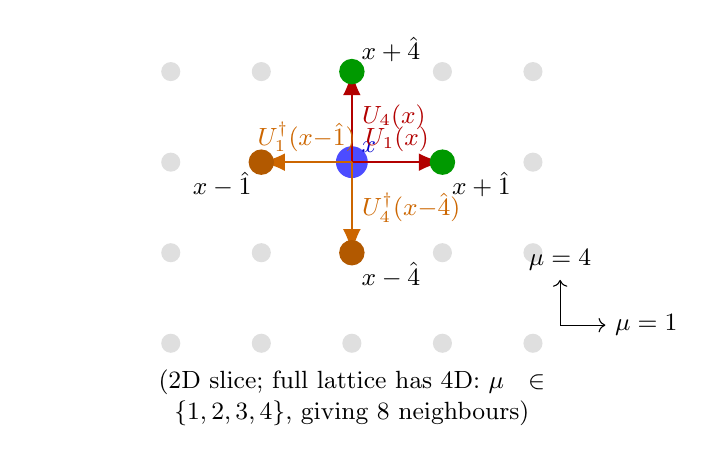
\begin{tikzpicture}[scale=1.15, font=\small]
  % Draw 2D slice of lattice (x-t plane)
  \foreach \x in {0,1,2,3,4} {
    \foreach \t in {0,1,2,3} {
      \fill[gray!25] (\x,\t) circle (3pt);
    }
  }
  % Highlight center site
  \fill[blue!70] (2,2) circle (5pt);
  \node[above right, blue!80!black] at (2,2) {$x$};
  % Forward links (arrows)
  \draw[-{Latex[length=3mm]}, thick, red!70!black]
    (2,2) -- (3,2) node[midway, above] {$U_1(x)$};
  \draw[-{Latex[length=3mm]}, thick, red!70!black]
    (2,2) -- (2,3) node[midway, right] {$U_4(x)$};
  % Backward links (dagger)
  \draw[-{Latex[length=3mm]}, thick, orange!80!black]
    (2,2) -- (1,2) node[midway, above] {$U_1^\dagger(x{-}\hat{1})$};
  \draw[-{Latex[length=3mm]}, thick, orange!80!black]
    (2,2) -- (2,1) node[midway, right] {$U_4^\dagger(x{-}\hat{4})$};
  % Neighbour labels
  \fill[green!60!black] (3,2) circle (4pt);
  \node[below right] at (3,2) {$x+\hat{1}$};
  \fill[green!60!black] (2,3) circle (4pt);
  \node[above right] at (2,3) {$x+\hat{4}$};
  \fill[orange!70!black] (1,2) circle (4pt);
  \node[below left] at (1,2) {$x-\hat{1}$};
  \fill[orange!70!black] (2,1) circle (4pt);
  \node[below right] at (2,1) {$x-\hat{4}$};
  % Axes labels
  \node[below] at (2,0) {};
  \draw[->] (4.3,0.2) -- (4.8,0.2) node[right] {$\mu=1$};
  \draw[->] (4.3,0.2) -- (4.3,0.7) node[above] {$\mu=4$};
  % Caption note
  \node[align=center, text width=8cm] at (2,-0.6)
    {(2D slice; full lattice has 4D: $\mu\in\{1,2,3,4\}$, giving 8 neighbours)};
\end{tikzpicture}
\caption{Nearest-neighbour hopping of the Wilson operator on a 2D slice of
the 4D lattice.
Site $x$ (blue) is connected to its 8 neighbours via forward gauge links
$U_\mu(x)$ (red) and backward links $U_\mu^\dagger(x-\hat\mu)$ (orange).
The forward hop carries the projector $(1-\gamma_\mu)$; the backward hop
carries $(1+\gamma_\mu)$.}
\label{fig:wilson_hopping}
\end{figure}

\subsubsection{Hopping Parameter and Critical Mass}

Increasing $\kappa$ corresponds to decreasing quark mass $m_0$.
There exists a critical value $\kappa_{\mathrm{crit}} \lesssim 1/8$ (shifted from
the free-field value by gauge interactions) at which the quark becomes
\textbf{massless} and $D_W$ becomes singular:
\begin{equation}
  \kappa(D_W) \;\sim\; \frac{1}{\kappa_{\mathrm{hop}} - \kappa_{\mathrm{crit}}},
  \qquad \kappa_{\mathrm{hop}} \to \kappa_{\mathrm{crit}}.
  \label{eq:wilson_condition}
\end{equation}
Physical simulations target $\kappa_{\mathrm{hop}}$ close to $\kappa_{\mathrm{crit}}$
to reproduce light quark masses, making the system inherently ill-conditioned.
This is the primary numerical challenge that motivates multi-word arithmetic.

\subsubsection{Non-Hermiticity and Solver Choice}

The Wilson operator satisfies $\gamma_5 D_W \gamma_5 = D_W^\dagger$
(\textbf{$\gamma_5$-Hermiticity}), but $D_W \neq D_W^\dagger$, so
standard CG is inapplicable.
Two solver strategies are used:
\begin{itemize}
  \item \textbf{BiCGStab} applied directly to $D_W\psi = b$ (non-symmetric):
        2 SpMV applications of $D_W$ per iteration.
  \item \textbf{CG} applied to the Hermitian system $(D_W^\dagger D_W)\psi = D_W^\dagger b$:
        the normal equations, but this squares $\kappa(D_W)$.
\end{itemize}
BiCGStab is the standard choice for Wilson fermions in practice.

\subsubsection{Clover (Sheikholeslami--Wohlert) Improvement}

The Wilson term breaks chiral symmetry and introduces $O(a)$ discretization
errors.
The Clover improvement~\cite{Akahoshi2022} adds a second term:
\begin{equation}
  D_{\mathrm{clover}}(x,x) = \delta_{x,x} - \tfrac{i}{4}\,c_{SW}\,\kappa
    \sum_{\mu<\nu} \sigma_{\mu\nu} F_{\mu\nu}(x),
  \label{eq:clover}
\end{equation}
where $\sigma_{\mu\nu} = \tfrac{i}{2}[\gamma_\mu,\gamma_\nu]$ and $F_{\mu\nu}$
is the clover-leaf approximation to the field strength tensor.
This removes $O(a)$ errors, leaving only $O(a^2)$ artifacts.
The Clover term is \textbf{diagonal in site index}---it does not add new
off-diagonal entries---so it modifies the diagonal block $D_{ee/oo}$ in
even-odd preconditioning (Section~\ref{sec:evenodd}) without changing the
hopping structure.

% ----------------------------------------------------------
\subsection{Domain-Wall Fermion Operator}
\label{sec:dwf}

\subsubsection{Motivation: Preserving Chiral Symmetry}

Chiral symmetry---the invariance of massless QCD under independent phase
rotations of left- and right-handed quark fields---plays a fundamental role
in hadron physics.
The Wilson term explicitly breaks chiral symmetry, leading to unwanted
additive mass renormalizations.
Domain-Wall Fermions~\cite{Kaplan1992,Shamir1993} recover chiral symmetry
on the lattice by a geometric construction: the quark field propagates
in a \textbf{5-dimensional slab}, and chiral modes emerge as
zero-modes \emph{trapped on the 4D boundaries}.

\subsubsection{The 5D Operator: Shamir Variant}

The DWF operator extends the 4D lattice with a 5th direction $s \in \{0,\ldots,L_s-1\}$,
giving a total field space of dimension $N_c \cdot N_d \cdot V \cdot L_s$:
\begin{equation}
  D_{\mathrm{DW}}(x,s;\,y,t)
  = D_W^{(4)}(x,y)\,\delta_{s,t}
  + \delta_{x,y}\,D_s(s,t),
  \label{eq:dwf_op}
\end{equation}
where $D_W^{(4)}$ is the 4D Wilson hopping operator (applied uniformly across
all $s$-slices), and $D_s$ governs propagation in the 5th direction.
In the Shamir formulation~\cite{Shamir1993}:
\begin{equation}
  D_s(s,t) = \begin{cases}
  P_- \,\delta_{t,s+1} + P_+ \,\delta_{t,s-1} & 0 < s < L_s-1 \\
  -m_f P_- \,\delta_{t,0} + P_+ \,\delta_{t,1} & s = 0 \\
  P_- \,\delta_{t,L_s-2} - m_f P_+ \,\delta_{t,L_s-1} & s = L_s-1
  \end{cases}
  \label{eq:ds_matrix}
\end{equation}
where $P_\pm = \tfrac{1}{2}(1\pm\gamma_5)$ are \textbf{chiral projectors} and
$m_f$ is the bare quark mass ($m_f \to 0$ for massless quarks).
The bulk coupling moves right-handed modes ($P_-$ in the $+s$ direction)
and left-handed modes ($P_+$ in the $-s$ direction), trapping them
on opposite walls.

\begin{figure}[H]
\centering
% Slab positions: s=0->x=0, s=1->x=1.55, ... s=5->x=7.75
% Slab width=1.3, height H=1.6
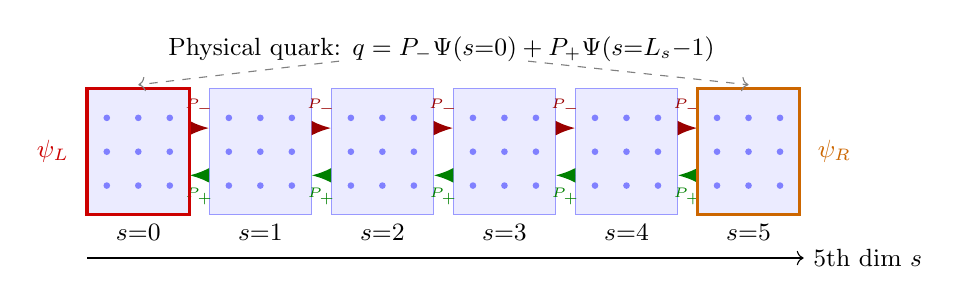
\begin{tikzpicture}[scale=1.0, font=\small]
  % Slabs s=0..5
  \foreach \xpos/\slabel in
    {0.00/0, 1.55/1, 3.10/2, 4.65/3, 6.20/4, 7.75/5} {
    \draw[fill=blue!8, draw=blue!40] (\xpos,0) rectangle (\xpos+1.3,1.6);
    \foreach \ii in {0.25, 0.65, 1.05} {
      \foreach \jj in {0.37, 0.80, 1.23} {
        \fill[blue!50] (\xpos+\ii, \jj) circle (1.2pt);
      }
    }
    \node[below] at (\xpos+0.65, 0) {\small $s{=}\slabel$};
  }
  % 5th-dim arrows between slabs (hardcoded xfrom = xpos+1.3, xto = xpos+1.55)
  \foreach \xf/\xt in
    {1.30/1.55, 2.85/3.10, 4.40/4.65, 5.95/6.20, 7.50/7.75} {
    \draw[-{Latex[length=2.5mm]}, thick, red!60!black]
      (\xf, 1.1) -- (\xt, 1.1) node[midway, above=1pt, font=\tiny] {$P_-$};
    \draw[-{Latex[length=2.5mm]}, thick, green!50!black]
      (\xt, 0.5) -- (\xf, 0.5) node[midway, below=1pt, font=\tiny] {$P_+$};
  }
  % Left boundary wall highlight
  \draw[very thick, red!80!black] (0,0) rectangle (1.3,1.6);
  \node[below=8pt, red!80!black, font=\bfseries\small] at (0.65, 0) {};
  \node[left=3pt, red!80!black] at (0, 0.8) {$\psi_L$};
  % Right boundary wall highlight
  \draw[very thick, orange!80!black] (7.75,0) rectangle (9.05,1.6);
  \node[right=3pt, orange!80!black] at (9.05, 0.8) {$\psi_R$};
  % 5th-dim axis
  \draw[->] (0,-0.55) -- (9.1,-0.55) node[right] {5th dim $s$};
  % Physical quark annotation
  \node[align=center, font=\small] at (4.5, 2.1)
    {Physical quark: $q = P_-\Psi(s{=}0) + P_+\Psi(s{=}L_s{-}1)$};
  \draw[->, dashed, gray] (3.2, 1.95) -- (0.65, 1.65);
  \draw[->, dashed, gray] (5.6, 1.95) -- (8.4,  1.65);
\end{tikzpicture}
\caption{Domain-Wall Fermion structure.
The 4D lattice is extended to $L_s$ slices in the 5th direction.
Right-handed modes ($P_-$, red arrows) propagate toward $s=0$;
left-handed modes ($P_+$, green arrows) propagate toward $s=L_s-1$.
They are exponentially localised on opposite walls with amplitude
$\sim e^{-\alpha s}$ (left wall) and $\sim e^{-\alpha(L_s-1-s)}$ (right wall).
The physical 4D quark propagator is obtained by projecting the solution
onto the boundary walls.}
\label{fig:dwf_structure}
\end{figure}

\subsubsection{Physical Solution Extraction}

The 5D system is solved for the full field $\Psi(x,s)$, and the
physical quark propagator is obtained by the boundary projections:
\begin{equation}
  q(x) = P_-\,\Psi(x,0) + P_+\,\Psi(x,L_s-1),
  \qquad
  \bar{q}(x) = \bar\Psi(x,0)\,P_+ + \bar\Psi(x,L_s-1)\,P_-.
\end{equation}
The chiral symmetry breaking is residual:
\begin{equation}
  m_{\mathrm{res}} \;\sim\; e^{-\alpha L_s},
\end{equation}
where $\alpha > 0$ depends on the gap in the 5D spectrum.
Increasing $L_s$ exponentially suppresses the explicit chiral symmetry
breaking, at the cost of an $L_s$-fold increase in computational expense.

\subsubsection{Solver: CGNE and the Squared Condition Number}

The DWF operator is $\gamma_5$-Hermitian in a generalised sense, but not
symmetric positive-definite.
The standard approach applies \textbf{CGNE} (CG on the Normal Equations):
\begin{equation}
  D_{\mathrm{DW}}^\dagger D_{\mathrm{DW}}\, x = D_{\mathrm{DW}}^\dagger b.
  \label{eq:normal_eq}
\end{equation}
The matrix $A = D_{\mathrm{DW}}^\dagger D_{\mathrm{DW}}$ is SPD with condition number:
\begin{equation}
  \kappa(A) = \kappa(D_{\mathrm{DW}}^\dagger D_{\mathrm{DW}})
  = \kappa(D_{\mathrm{DW}})^2.
  \label{eq:kappa_squared}
\end{equation}
This squaring is the central numerical difficulty: near the chiral limit,
$\kappa(D_{\mathrm{DW}}) \sim 10^6$--$10^{12}$, so
$\kappa(A) \sim 10^{12}$--$10^{24}$---far beyond what FP64 can handle.

\begin{tcolorbox}[warnbox={Why DWF Is Harder Than Wilson}]
\begin{tabular}{lll}
 & \textbf{Wilson + BiCGStab} & \textbf{DWF + CGNE} \\
\hline
Matrix condition & $\kappa(D_W)$ & $\kappa(D_W)^2$ \\
SpMV per iter   & 2 ($D_W$ only) & 2 ($D_{\mathrm{DW}}$ and $D_{\mathrm{DW}}^\dagger$) \\
Slab cost       & $V$ sites      & $L_s \cdot V$ sites \\
Total overhead  & $1\times$ (baseline) & $\sim L_s \times \kappa$-amplified \\
\end{tabular}

\medskip
Both the squared condition number and the $L_s$-fold operator cost make
DWF+CGNE the primary target for QDW/QTW arithmetic.
\end{tcolorbox}

\subsubsection{M\"{o}bius Domain-Wall Fermions}

The M\"{o}bius variant~\cite{Brower2012} replaces the Shamir kernel
with a rational approximation to the sign function:
\begin{equation}
  D_{\mathrm{M\ddot{o}b}}^{5D} = \frac{D_{\mathrm{DW}}(\omega_n)}{1+D_{\mathrm{DW}}(\omega_n)},
\end{equation}
where $\omega_n$ are optimised coefficients.
This achieves the same chiral accuracy as Shamir DWF with a smaller $L_s$,
reducing computational cost while maintaining the 5D structure and CGNE solver.
Related work from this group~\cite{Chen2026} further modifies the 5D coupling
$D_s$ to improve the condition number of the normal equations while leaving the
4D physical solution unchanged.

% ----------------------------------------------------------
\subsection{Even-Odd (Checkerboard) Preconditioning}
\label{sec:evenodd}

Both Wilson and DWF operators can be substantially accelerated by
\textbf{even-odd preconditioning} (checkerboard decomposition), which
reduces the effective matrix size by a factor of 2.

\subsubsection{Site Decomposition}

Lattice sites are partitioned into \textbf{even} and \textbf{odd} sublattices
by site coordinate parity:
\begin{equation}
  \text{even}: (x_0+x_1+x_2+x_3) \bmod 2 = 0, \qquad
  \text{odd}:  (x_0+x_1+x_2+x_3) \bmod 2 = 1.
\end{equation}
Since the hopping term only connects nearest neighbours, the Wilson
operator has a block structure:
\begin{equation}
  D_W =
  \begin{pmatrix}
    D_{ee} & D_{eo} \\
    D_{oe} & D_{oo}
  \end{pmatrix},
  \label{eq:block_D}
\end{equation}
where $D_{ee}$ and $D_{oo}$ are purely diagonal (mass terms, no hopping),
and $D_{eo}$, $D_{oe}$ are the off-diagonal hopping terms.

\begin{figure}[H]
\centering
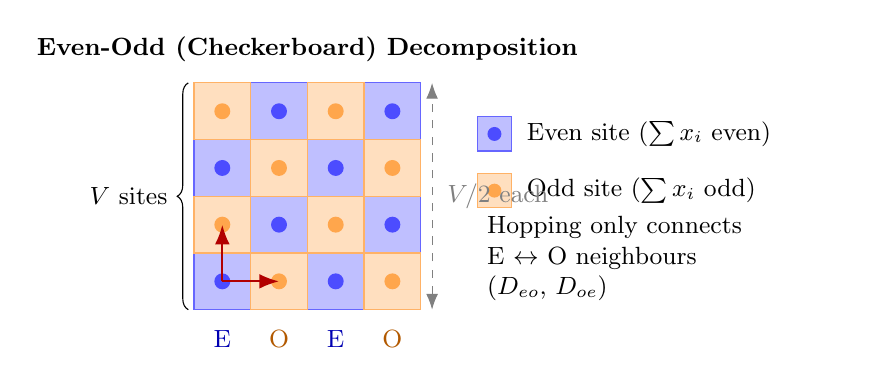
\begin{tikzpicture}[scale=0.72, font=\small]
  % Draw 4x4 checkerboard (even = blue, odd = orange)
  % Even squares (x+y even)
  \foreach \x/\y in {0/0,0/2,1/1,1/3,2/0,2/2,3/1,3/3} {
    \draw[fill=blue!25, draw=blue!60] (\x,\y) rectangle (\x+1,\y+1);
    \fill[blue!70] (\x+0.5,\y+0.5) circle (4pt);
  }
  % Odd squares (x+y odd)
  \foreach \x/\y in {0/1,0/3,1/0,1/2,2/1,2/3,3/0,3/2} {
    \draw[fill=orange!25, draw=orange!60] (\x,\y) rectangle (\x+1,\y+1);
    \fill[orange!70] (\x+0.5,\y+0.5) circle (4pt);
  }
  % Hopping arrow: even -> odd
  \draw[-{Latex[length=2.5mm]}, thick, red!70!black]
    (0.5,0.5) -- (1.5,0.5);
  \draw[-{Latex[length=2.5mm]}, thick, red!70!black]
    (0.5,0.5) -- (0.5,1.5);
  % Labels
  \node[above] at (2,4.2) {\textbf{Even-Odd (Checkerboard) Decomposition}};
  \node[below] at (0.5, -0.2) {\color{blue!70!black}E};
  \node[below] at (1.5, -0.2) {\color{orange!70!black}O};
  \node[below] at (2.5, -0.2) {\color{blue!70!black}E};
  \node[below] at (3.5, -0.2) {\color{orange!70!black}O};
  % Legend
  \fill[blue!25, draw=blue!60] (5.0,2.8) rectangle (5.6,3.4);
  \fill[blue!70] (5.3, 3.1) circle (3.5pt);
  \node[right] at (5.7, 3.1) {Even site ($\sum x_i$ even)};
  \fill[orange!25, draw=orange!60] (5.0,1.8) rectangle (5.6,2.4);
  \fill[orange!70] (5.3, 2.1) circle (3.5pt);
  \node[right] at (5.7, 2.1) {Odd site ($\sum x_i$ odd)};
  % Hopping note
  \node[right, align=left, text width=4.5cm] at (5.0, 0.9)
    {\small Hopping only connects\\E $\leftrightarrow$ O neighbours\\($D_{eo}$, $D_{oe}$)};
  % Size annotation
  \draw[decorate, decoration={brace,amplitude=4pt}] (-0.1,0) -- (-0.1,4)
    node[midway, left=4pt] {$V$ sites};
  \draw[{Latex[length=2mm]}-{Latex[length=2mm]}, dashed, gray] (4.2,0) -- (4.2,4)
    node[midway, right=2pt, gray] {\small $V/2$ each};
\end{tikzpicture}
\caption{Even-odd (checkerboard) decomposition of the lattice.
Blue sites (even: $\sum_\mu x_\mu$ even) and orange sites (odd) form two sublattices.
Nearest-neighbour hopping only connects even $\leftrightarrow$ odd sites, giving the
block off-diagonal structure~\eqref{eq:block_D}.
Each sublattice contains $V/2$ sites, and the Schur-complement system~\eqref{eq:schur}
acts only on the even sublattice.}
\label{fig:checkerboard}
\end{figure}

\subsubsection{Schur Complement}

Applying the Schur decomposition to~\eqref{eq:block_D}:
\begin{equation}
  \hat{D} \;=\; D_{ee} - D_{eo}\,D_{oo}^{-1}\,D_{oe}.
  \label{eq:schur}
\end{equation}
Since $D_{oo}$ is diagonal, $D_{oo}^{-1}$ is trivially computed in $O(V/2)$.

\subsubsection{Reduced System}

The full solve $D_W \psi = b$ reduces to solving the \emph{half-size} system:
\begin{equation}
  \hat{D}\,\psi_e = b_e - D_{eo}D_{oo}^{-1}b_o \;\eqqcolon\; \hat{b}_e,
  \label{eq:reduced}
\end{equation}
followed by the trivial recovery of the odd-site solution:
\begin{equation}
  \psi_o = D_{oo}^{-1}(b_o - D_{oe}\,\psi_e).
\end{equation}

\subsubsection{Computational Benefit and DWF Extension}

The effective matrix $\hat{D}$ acts on $V/2$ sites.
One application of $\hat{D}$ requires two Wilson hoppings on half the sites,
so the net SpMV cost is equal to one full $D_W$ application, but the
\textbf{iteration count is roughly halved} due to improved diagonal dominance.

For DWF, the even-odd decomposition is applied in the 4D directions only;
the 5th-dimension coupling in $D_s$ is absorbed into the diagonal blocks
$D_{ee/oo}^{(5D)}$.
The Schur complement is formed analogously to~\eqref{eq:schur}.

\begin{tcolorbox}[keybox={Even-Odd and Multi-Word Arithmetic}]
The spinor fields $\psi_e$ in the reduced system~\eqref{eq:reduced} are the
natural target for QDW/QTW promotion.
With even-odd preconditioning, the extended spinor arrays have size $V/2$
rather than $V$, \textbf{halving the memory overhead} of QDW ($2\times$ memory)
and QTW ($3\times$ memory) relative to the full-lattice case.
\end{tcolorbox}

% ----------------------------------------------------------
\subsection{The Bridge++ Code Set}
\label{sec:bridgepp}

All numerical work is based on \textbf{Bridge++}~\cite{Bridge,Akahoshi2022},
a general-purpose Lattice QCD code set designed for portability, readability,
and performance across diverse HPC architectures.

\subsubsection{Design and GPU Backends}

Bridge++ is written in C++ with an object-oriented architecture.
Version 2.0~\cite{Akahoshi2022} introduced machine-dependent optimization
modules enabling flexible data layouts, SIMD vectorization, and GPU offloading.
Two GPU backends are available:
\begin{itemize}
  \item \textbf{OpenACC/OpenMP offload:} directive-based, portable across
        NVIDIA and AMD GPUs.
  \item \textbf{CUDA:} API-based, enables detailed hardware tuning.
\end{itemize}
A performance comparison of the two approaches is reported in~\cite{Chen2025}:
CUDA achieves higher peak performance; OpenACC approaches it at large volumes.

\subsubsection{Data Layout: AoSoA with Packing Width NWP}

The spinor field uses an \textbf{Array-of-Structures-of-Arrays (AoSoA)} layout
with packing width $\NWP = 32$ (matching the NVIDIA warp size):
\begin{equation}
  \mathrm{index}(\mathtt{ri},\, c,\, d,\, s,\, \mathtt{site})
  = (\mathtt{site}\;\%\;\NWP)
  + \NWP \times
  \bigl(\mathtt{ri} + 2(c + \Nc(d + \Nd(s + \Ns\,(\mathtt{site}/\NWP))))\bigr),
  \label{eq:bridge_index}
\end{equation}
where $\mathtt{ri} \in \{0,1\}$ indexes real/imaginary parts.
The $\NWP$ innermost sites form the warp unit; all 32 threads access
consecutive memory locations in a single coalesced transaction.
This layout is the starting point for DW/TW spinor extensions
in Section~\ref{sec:layout}.

\subsubsection{Available Solvers}

\begin{table}[H]
\centering
\caption{Iterative solvers in Bridge++ relevant to this work.}
\begin{tabular}{llll}
\toprule
\textbf{Solver} & \textbf{Applicable to} & \textbf{SpMV/iter} & \textbf{Notes} \\
\midrule
CG              & SPD matrices only       & 1  & Inapplicable to $D_W$ or $D_{\mathrm{DW}}$ \\
BiCGStab        & General non-Hermitian   & 2  & Standard for Wilson fermions \\
CGNE            & Non-SPD via $D^\dagger D$ & 2  & Standard for DWF \\
\bottomrule
\end{tabular}
\end{table}

\subsubsection{Related Precision Work on Bridge++}

Two companion papers directly motivate the present work.
Kanamori et al.~\cite{Kanamori2026} implement FP16 mixed-precision BiCGStab
for Wilson fermions on the A64FX (Fugaku), achieving near-FP64 convergence
with a per-iteration rescaling strategy analogous to QDW/QTW normalization.
Chen et al.~\cite{Chen2026} implement Neff's modified DWF operator~\cite{Neff2015}
in Bridge++, which algebraically reduces $\kappa(D_{\mathrm{DW}}^\dagger D_{\mathrm{DW}})$
and complements the arithmetic precision increase provided by QDW/QTW.


% ##########################################################
% CHAPTER 3: COMBINING MULTIWORD ARITHMETIC WITH LATTICE QCD
% ##########################################################

% ==========================================================
\section{Multi-Word Arithmetic in Lattice QCD Solvers}
\label{sec:application}

This chapter combines the arithmetic framework of Chapter~1 with the
Lattice QCD operators described in Chapter~2, and works out the
concrete implementation decisions required to deploy QDW/QTW in Bridge++.
Section~\ref{sec:cgne} presents the QDW/QTW CGNE algorithm with the
critical normalization step.
Section~\ref{sec:precision_assignment} analyses which quantities benefit
from precision promotion.
Section~\ref{sec:layout} describes GPU memory layouts for extended spinors.
Section~\ref{sec:lqcd_comparison} analyses the condition-number regime and
when each method is needed.
Section~\ref{sec:future} proposes a systematic $2\times3$ benchmark comparing
Wilson and DWF under FP64, QDW, and QTW.

% ----------------------------------------------------------
\subsection{CGNE Solver with QDW/QTW Precision}
\label{sec:cgne}

The normal equation system~\eqref{eq:normal_eq} for DWF
($D_{\mathrm{DW}}^\dagger D_{\mathrm{DW}}\,x = D_{\mathrm{DW}}^\dagger b$)
is solved by CGNE.
The squared condition number~\eqref{eq:kappa_squared} makes
FP64 precision insufficient near the chiral limit; QDW/QTW are applied to
the spinor vectors and scalar quantities within the solver.

\begin{algorithm}[H]
\caption{CGNE with QDW/QTW precision (Lattice QCD, DWF)}
\begin{algorithmic}[1]
\State $r \leftarrow b - D\,x_0$;\quad
       $p \leftarrow D^\dagger r$;\quad
       $\rho \leftarrow \mathrm{QDWdot}(r, r)$
\For{$k = 1, 2, \ldots$}
  \State $q \leftarrow \mathrm{QDW\text{-}SpMV}(D,\; p)$
    \Comment{Apply $D_{\mathrm{DW}}$ (dominant cost)}
  \State $\alpha \leftarrow \rho \;/\; \mathrm{QDWdot}(q, q)$
  \State $x \leftarrow x + \alpha\, p$
    \Comment{AXPY}
  \State $r \leftarrow r - \alpha\, q$
    \Comment{AXPY}
  \State $\boxed{r \leftarrow \mathrm{Normalize}(r)}$
    \Comment{{\color{red}Key: one normalization per iteration (Section~\ref{sec:drift})}}
  \State $\rho' \leftarrow \mathrm{QDWdot}(r, r)$
  \If{converged} \textbf{break} \EndIf
  \State $\beta \leftarrow \rho' / \rho$
  \State $p \leftarrow D^\dagger r + \beta\, p$
    \Comment{Apply $D^\dagger_{\mathrm{DW}}$ (second SpMV per iteration)}
  \State $\rho \leftarrow \rho'$
\EndFor
\end{algorithmic}
\end{algorithm}

\begin{remark}
The normalization on line 7 is applied once to the residual vector $r$
immediately after its AXPY update.
This single repair per iteration suppresses drift at negligible overhead
relative to SpMV, as established in Section~\ref{sec:drift}.
\end{remark}

% ----------------------------------------------------------
\subsection{Precision Assignment: Which Quantities Need DW?}
\label{sec:precision_assignment}

\subsubsection{Two Sources of Rounding Error in SpMV}

The SpMV $q = D\,p$ decomposes as:
\begin{equation}
  q = \sum_{\mu} U_\mu(\text{site}) \times \psi(\text{neighbour}),
\end{equation}
with rounding errors from two independent sources:

\begin{enumerate}
  \item \textbf{Matrix error (Source A):} error in $U_\mu$ from SU(3)
        reconstruction or finite-precision storage:
        $|U_{\mathrm{stored}} - U_{\mathrm{exact}}| = O(\uu \cdot |U|)$.

  \item \textbf{Accumulation error (Source B):} rounding accumulated over
        the sum $\sum_\mu$, growing with the number of terms $N$:
        FP64 dot $\langle r, r \rangle = \sum_i r_i^2 + O(N \cdot \uu \cdot \|r\|^2)$.
\end{enumerate}

DW arithmetic acts \textbf{only on Source B}.
Promoting spinors to DW reduces Source B from $O(N\uu)$ to $O(N\uu^2)$,
preventing the solver from stagnating when $\kappa(D)$ is large.
The achievable solution accuracy is ultimately bounded by:
\begin{equation}
  \text{solution error} \;\geq\; \kappa(D) \times O(\uu),
\end{equation}
regardless of spinor precision, because Source A (matrix error) is fixed.

\subsubsection{SU(3) Reconstruction: FP64 Is Sufficient}

The SU(3) gauge link is stored compressed (two rows, third reconstructed
via cross product $\text{row}_3 = \overline{\text{row}_1 \times \text{row}_2}$).
The reconstruction error $O(\uu \cdot |U|)$ is identical in order to storing
all three rows in FP64.
Promoting reconstruction to DW ($O(\uu^2)$) provides no benefit, since the
FP64 matrix already introduces $O(\uu)$ error regardless.

\subsubsection{Precision Assignment Table}

\begin{table}[H]
\centering
\caption{Recommended precision for each quantity in the CGNE solver.}
\begin{tabular}{llll}
\toprule
\textbf{Quantity} & \textbf{Precision} & \textbf{Reason} & \textbf{Error source} \\
\midrule
Spinor $\psi$, $p$    & \textbf{QDW/QTW} & Accumulation in dot/AXPY & Source B \\
Residual $r$          & \textbf{QDW/QTW} & $\alpha$, $\beta$, convergence check & Source B \\
Dot products          & \textbf{QDW/QTW} & Most sensitive to cancellation & Source B \\
Gauge link $U_\mu$    & FP64             & Matrix error already $O(\uu)$ & Source A \\
SU(3) reconstruction  & FP64             & Same order as storage error & Source A \\
\bottomrule
\end{tabular}
\end{table}

\subsubsection{Error Flow Through SpMV}

\begin{equation}
  \underbrace{U_\mu}_{\text{FP64},\; O(\uu)}
  \;\times\;
  \underbrace{\psi}_{\text{QDW},\; O(\uu^2)}
  \;\longrightarrow\;
  \underbrace{q}_{\text{element precision} \;=\; O(\uu)}
\end{equation}

Individual elements of $q$ are only FP64-accurate, but the
\emph{dot product} $\langle q, q \rangle$ computed in QDW still benefits:
\begin{align}
  \text{FP64 dot:}\quad \langle q, q \rangle &= \sum_i q_i^2 + O(N\uu\|q\|^2), \\
  \text{QDW dot:}\quad  \langle q, q \rangle &= \sum_i q_i^2 + O(N\uu^2\|q\|^2).
\end{align}
This is why QDW helps even when $U$ remains in FP64:
the \emph{aggregation} in inner products is where precision improvement matters.

% ----------------------------------------------------------
\subsection{Memory Layout for GPU Implementation}
\label{sec:layout}

\subsubsection{Existing Spinor Layout (AoSoA)}

The existing Bridge++ layout uses the index function~\eqref{eq:bridge_index}:
\begin{equation}
  \mathrm{index}(\mathtt{ri},\, c,\, d,\, s,\, \mathtt{site})
  = (\mathtt{site}\;\%\;\NWP)
  + \NWP \times
  \Bigl(\mathtt{ri} + 2\bigl(c + \Nc(d + \Nd(s + \Ns\,(\mathtt{site}/\NWP)))\bigr)\Bigr).
\end{equation}

\subsubsection{Three Options for DW Extension}

\textbf{Option A: Extend \texttt{ri} from 2 to 4}

Assign $\mathtt{ri} \in \{0,1,2,3\}$ as $\{r_{hi}, i_{hi}, r_{lo}, i_{lo}\}$.
Only the prefactor changes from 2 to 4.
\textit{Pros:} minimal change. \textit{Cons:} $hi$ and $lo$ are not adjacent.

\textbf{Option B: Separate hi/lo Arrays (SoA)}

Keep the existing layout for $hi$; allocate a second buffer for $lo$ with
the same index function.
\begin{lstlisting}[language=C++]
struct DWSpinorField {
    double *hi;  // existing buffer (size = total elements)
    double *lo;  // companion buffer (same size)
    // Same index() for both
};
\end{lstlisting}
\textit{Pros:} easy FP64 fallback; existing kernels untouched.
\textit{Cons:} two pointer arguments; doubled memory.

\textbf{Option C: \texttt{double4} Layout (Recommended for QDW)}

A DW complex spinor = 4 doubles = one CUDA \texttt{double4} (32 bytes):
\begin{equation}
  \texttt{double4}\;\{x,y,z,w\} = \{r_{hi},\; i_{hi},\; r_{lo},\; i_{lo}\}.
  \label{eq:double4_layout}
\end{equation}
Ordering $\{r_{hi}, i_{hi}, r_{lo}, i_{lo}\}$ (hi-words first) is preferred:
\begin{itemize}
  \item SpMV accesses $r_{hi}$ and $i_{hi}$ together (same \texttt{double4}).
  \item FP64 fallback: ignore \texttt{.z}, \texttt{.w}.
  \item Normalization symmetry: TwoSum on $(\texttt{.x},\texttt{.z})$
        and $(\texttt{.y},\texttt{.w})$.
\end{itemize}
With $\NWP = 32$: 32 threads $\times$ 32 bytes = 1024 bytes per transaction,
fully coalesced.
New index function (with \texttt{ri} absorbed into \texttt{double4}):
\begin{equation}
  \mathrm{index}_{\texttt{d4}}(c,\, d,\, s,\, \mathtt{site})
  = (\mathtt{site}\;\%\;\NWP)
  + \NWP \times
  \bigl(c + \Nc(d + \Nd(s + \Ns\,(\mathtt{site}/\NWP)))\bigr).
  \label{eq:d4_index}
\end{equation}

\subsubsection{QTW Layout: SoA $\times$ 3 (Recommended for QTW)}

A QTW complex spinor = 6 doubles (hi, mid, lo). The three separate-buffer
approach is recommended:
\begin{lstlisting}[language=C++]
struct QTWSpinorField {
    double2 *hi_buf;   // {r_hi, i_hi} x N
    double2 *mid_buf;  // {r_mid, i_mid} x N
    double2 *lo_buf;   // {r_lo, i_lo} x N
    // Same index for all three: index(c,d,s,site)
};
\end{lstlisting}
Each buffer: 32 threads $\times$ 16 bytes = 512 bytes per warp, fully coalesced.
An alternative 48-byte struct is rejected: 48 bytes = 1.5 $\times$ 32-byte
transactions causes alignment issues.

\subsubsection{Layout Comparison}

\begin{table}[H]
\centering
\caption{Memory layout strategies for DW and QTW spinor fields.}
\begin{tabular}{lcccc}
\toprule
 & \textbf{Option A} & \textbf{Option B (SoA)} & \textbf{Option C (double4)} & \textbf{QTW (SoA$\times$3)} \\
\midrule
Target precision        & DW   & DW   & DW/QDW & QTW \\
Coalesced $hi$ access   & Yes  & Yes  & Yes    & Yes \\
Coalesced $lo/mid$ access & Yes & Yes  & Yes    & Yes \\
FP64 fallback ease      & Mod  & Easy & Easy   & Moderate \\
Words per complex spinor & 4   & 4    & 4      & 6 \\
Memory overhead         & $2\times$ & $2\times$ & $2\times$ & $3\times$ \\
\bottomrule
\end{tabular}
\end{table}

\subsubsection{CUDA Kernel: QDW Hopping with \texttt{double4}}
\label{sec:double4}

\begin{lstlisting}[language=C++, caption={QDW hopping kernel using \texttt{double4} (Bridge++ style, NWP=32)}]
// Layout: double4 = {r_hi, i_hi, r_lo, i_lo}

__device__ __forceinline__
void two_sum(double a, double b, double &s, double &e) {
    s = a + b;
    double v = s - a;
    e = (a - (s - v)) + (b - v);
}

__device__ __forceinline__
void two_prod(double a, double b, double &p, double &e) {
    p = a * b;
    e = __fma_rn(a, b, -p);   // CUDA native FMA
}

__global__ void qdw_hopping_kernel(
    double4* __restrict__ out,
    const double4* __restrict__ in,
    const double2* __restrict__ gauge,  // SU(3) link in FP64 (not DW)
    int NWP, int Nc, int Nd, int Ns)
{
    int lane       = threadIdx.x % NWP;
    int site_block = blockIdx.x;

    for (int d = 0; d < Nd; d++) {
    for (int c = 0; c < Nc; c++) {
        int idx = lane + NWP*(c + Nc*(d + Nd*(0 + Ns*site_block)));
        double4 psi = in[idx];
        double r_hi = psi.x, i_hi = psi.y;
        double r_lo = psi.z, i_lo = psi.w;

        double2 U = gauge[/*neighbor index*/0];
        double u_r = U.x, u_i = U.y;

        // QDW complex multiply: out = U * psi
        double p_rr, e_rr;  two_prod(u_r, r_hi, p_rr, e_rr);
        double p_ii, e_ii;  two_prod(u_i, i_hi, p_ii, e_ii);
        double p_ri, e_ri;  two_prod(u_r, i_hi, p_ri, e_ri);
        double p_ir, e_ir;  two_prod(u_i, r_hi, p_ir, e_ir);

        double out_r_hi, out_r_e;
        two_sum(p_rr, -p_ii, out_r_hi, out_r_e);
        double out_r_lo = out_r_e + (e_rr - e_ii) + (u_r*r_lo - u_i*i_lo);

        double out_i_hi, out_i_e;
        two_sum(p_ri, p_ir, out_i_hi, out_i_e);
        double out_i_lo = out_i_e + (e_ri + e_ir) + (u_r*i_lo + u_i*r_lo);

        out[idx] = make_double4(out_r_hi, out_i_hi, out_r_lo, out_i_lo);
    }}
}

// Normalization kernel: called ONCE per CGNE iteration
__global__ void normalize_spinor_dw(double4* spinor, int N) {
    int i = blockIdx.x * blockDim.x + threadIdx.x;
    if (i >= N) return;
    double4 s = spinor[i];
    double sr, er, si, ei;
    two_sum(s.x, s.z, sr, er);   // real:  (r_hi, r_lo) -> normalized
    two_sum(s.y, s.w, si, ei);   // imag:  (i_hi, i_lo) -> normalized
    spinor[i] = make_double4(sr, si, er, ei);
}
\end{lstlisting}

\subsubsection{CUDA Kernel: QTW Normalization with SoA$\times$3}

\begin{lstlisting}[language=C++, caption={QTW normalization kernel using SoA$\times$3}]
__global__ void normalize_qtw(
    double2* hi_buf, double2* mid_buf, double2* lo_buf, int N)
{
    int i = blockIdx.x * blockDim.x + threadIdx.x;
    if (i >= N) return;
    double2 hi = hi_buf[i], mid = mid_buf[i], lo = lo_buf[i];

    // Renormalize real: (hi.x, mid.x, lo.x)
    double s1r, e1r; two_sum(mid.x, lo.x, s1r, e1r);
    double zhr, tr;  two_sum(hi.x, s1r, zhr, tr);
    double zmr, zlr; two_sum(tr, e1r, zmr, zlr);

    // Renormalize imag: (hi.y, mid.y, lo.y)
    double s1i, e1i; two_sum(mid.y, lo.y, s1i, e1i);
    double zhi, ti;  two_sum(hi.y, s1i, zhi, ti);
    double zmi, zli; two_sum(ti, e1i, zmi, zli);

    hi_buf[i]  = make_double2(zhr, zhi);
    mid_buf[i] = make_double2(zmr, zmi);
    lo_buf[i]  = make_double2(zlr, zli);
}
\end{lstlisting}

% ----------------------------------------------------------
\subsection{Condition Number Analysis}
\label{sec:lqcd_comparison}

\subsubsection{Why Lattice QCD Differs from General SpMV}

The Mukunoki \& Ozaki~\cite{Mukunoki2025} experiments used general sparse
matrices on CPU.
The Lattice QCD setting differs in two important ways:
\begin{enumerate}
  \item \textbf{Condition number is systematically large and physics-controlled.}
        For DWF: $\kappa(D_{\mathrm{DW}}^\dagger D_{\mathrm{DW}}) = \kappa(D_{\mathrm{DW}})^2$,
        growing systematically as $\kappa \to \kappa_{\mathrm{crit}}$.
        This is not accidental---it is an inherent feature of the chiral limit.

  \item \textbf{The matrix is never stored; the inner product sum is short.}
        Only 8 nearest neighbours in 4D contribute to each site's SpMV.
        The accumulation sum is short compared to general SpMV,
        which changes the relative importance of Sources A and B.
\end{enumerate}

\subsubsection{Effective Precision Thresholds}

Define the effective rounding unit after $N$-term accumulation:
\begin{align}
  \uu_{\mathrm{eff}}^{(\mathrm{FP64})} &= N \cdot \uu \approx 10^6 \times 10^{-16} = 10^{-10}, \\
  \uu_{\mathrm{eff}}^{(\mathrm{QDW})}  &= N \cdot \uu^2 \approx 10^6 \times 10^{-32} = 10^{-26}, \\
  \uu_{\mathrm{eff}}^{(\mathrm{QTW})}  &= N \cdot \uu^3 \approx 10^6 \times 10^{-48} = 10^{-42}.
\end{align}

Stagnation occurs when $\uu_{\mathrm{eff}} \times \kappa(D^\dagger D) \gtrsim 1$:

\begin{table}[H]
\centering
\caption{Approximate stagnation thresholds ($N = 10^6$).
         $\checkmark$ = converges, $\times$ = stagnates.}
\begin{tabular}{lcccc}
\toprule
$\kappa(D)$ & $\kappa(D^\dagger D)$ & FP64 & QDW & QTW \\
\midrule
$10^5$    & $10^{10}$ & $\checkmark$ & $\checkmark$ & $\checkmark$ \\
$10^7$    & $10^{14}$ & $\times$ (slow) & $\checkmark$ & $\checkmark$ \\
$10^9$    & $10^{18}$ & $\times$        & $\checkmark$ & $\checkmark$ \\
$10^{13}$ & $10^{26}$ & $\times$        & $\times$     & $\checkmark$ \\
\bottomrule
\end{tabular}
\end{table}

The regime $\kappa(D) \gtrsim 10^{13}$ is where QDW stagnates and QTW becomes
the only viable option.
Whether this regime is encountered depends on the gauge configuration and $\kappa$.

\begin{tcolorbox}[warnbox={Implementation Order}]
\begin{enumerate}
  \item \textbf{Implement QDW first} (\texttt{double4} layout, 2$\times$ memory).
        Smallest code change; may already be sufficient.
  \item \textbf{Implement QTW only if} QDW stagnates at physically relevant
        $\kappa$ values, or total-time benchmarks show QTW to be faster.
  \item The threshold $\kappa^{**}$ where QDW stagnates is \textbf{empirical}
        and cannot be predicted from theory alone.
\end{enumerate}
\end{tcolorbox}

% ----------------------------------------------------------
\subsection{Future Research: Systematic Wilson vs DWF Benchmark}
\label{sec:future}

\subsubsection{The $2 \times 3$ Benchmark Matrix}

The central open question is whether, and under what conditions, QDW or QTW
provide a meaningful speedup for each fermion formulation.
We propose a systematic $2 \times 3$ benchmark:

\begin{table}[H]
\centering
\caption{Proposed benchmark matrix.
         Each cell records: total wall time $T$, iteration count $K$,
         and final relative residual $\|r\|/\|b\|$.}
\begin{tabular}{lccc}
\toprule
 & \textbf{FP64} & \textbf{QDW} & \textbf{QTW} \\
\midrule
\textbf{Wilson (BiCGStab)}  & $T_{W,64},\;K_{W,64}$ & $T_{W,Q2},\;K_{W,Q2}$ & $T_{W,Q3},\;K_{W,Q3}$ \\
\textbf{DWF (CGNE)}         & $T_{D,64},\;K_{D,64}$ & $T_{D,Q2},\;K_{D,Q2}$ & $T_{D,Q3},\;K_{D,Q3}$ \\
\bottomrule
\end{tabular}
\end{table}

\subsubsection{Predicted Behaviour and Hypotheses}

\begin{table}[H]
\centering
\caption{Predicted behaviour per cell.
         ``$\downarrow K$'' = iteration count reduction relative to FP64.}
\begin{tabular}{lll}
\toprule
 & \textbf{Wilson + BiCGStab} & \textbf{DWF + CGNE} \\
\midrule
FP64 & Converges for moderate $\kappa$; & Stagnates earlier ($\kappa^2$); \\
     & stagnates near $m_{\mathrm{crit}}$ & often the current bottleneck \\[4pt]
QDW  & Moderate $\downarrow K$; & Larger $\downarrow K$; \\
     & overhead $\approx 1.3\times$ likely absorbed & QDW may already be sufficient \\[4pt]
QTW  & $\downarrow K$ over QDW small; & $\downarrow K$ over QDW likely significant; \\
     & total time may increase & QTW may win on total time \\
\bottomrule
\end{tabular}
\end{table}

Testable hypotheses:
\begin{enumerate}
  \item \textbf{H1 (DWF benefits more):} The squared condition number means
        QDW/QTW provide larger iteration-count reduction for DWF+CGNE than
        for Wilson+BiCGStab.

  \item \textbf{H2 (QTW crossover for DWF):} There exists $\kappa^{**}$ near
        $\kappa_{\mathrm{crit}}$ where QTW achieves shorter total wall time
        than QDW for DWF+CGNE, as the iteration reduction outweighs the
        $\approx 1.85\times$ per-iteration overhead difference.

  \item \textbf{H3 (Wilson may not need QTW):} For Wilson+BiCGStab at typical
        parameters, QDW suffices and QTW provides no total-time benefit.
\end{enumerate}

\subsubsection{Implementation Plan}

\begin{table}[H]
\centering
\caption{Implementation checklist.}
\begin{tabular}{clll}
\toprule
\textbf{Step} & \textbf{Task} & \textbf{Layout} & \textbf{Notes} \\
\midrule
1 & FP64 BiCGStab (Wilson)   & existing \texttt{double2} AoSoA & baseline \\
2 & FP64 CGNE (DWF)          & same                             & baseline \\
3 & QDW BiCGStab              & \texttt{double4}, Eq.~\eqref{eq:d4_index} & Section~\ref{sec:double4} \\
4 & QDW CGNE                  & same                             & \\
5 & QTW BiCGStab              & SoA $\times 3$ (hi/mid/lo)       & Section~\ref{sec:layout} \\
6 & QTW CGNE                  & same                             & \\
\bottomrule
\end{tabular}
\end{table}

\subsubsection{Metrics and Analysis}

For each configuration, record across a range of $\kappa$ values:
total wall time $T$, iteration count $K$, per-iteration time $T/K$,
final residual $\|r\|/\|b\|$, and GPU memory footprint.
The crossing points $\kappa^*$ (FP64 stagnates) and $\kappa^{**}$
(QDW stagnates / QTW becomes faster) are the primary observables.

\begin{tcolorbox}[keybox={Why This Benchmark Matters}]
This is the first systematic evaluation of quasi multi-word arithmetic
in GPU-accelerated Lattice QCD solvers, covering both Wilson (BiCGStab)
and DWF (CGNE) formulations.
It occupies a distinct region of the precision-performance design space
from both~\cite{Kanamori2026} (FP16, lower precision) and~\cite{Chen2026}
(Neff's operator, algebraic $\kappa$ reduction).
The Bridge++ codebase~\cite{Chen2025} provides a unified framework making
a controlled $2\times3$ comparison feasible.
\end{tcolorbox}


% ##########################################################
% REFERENCES
% ##########################################################

\section*{References}
\addcontentsline{toc}{section}{References}

\begin{thebibliography}{99}

\bibitem{Knuth1969}
D.~E. Knuth,
\textit{The Art of Computer Programming, Vol.~2: Seminumerical Algorithms},
Addison-Wesley, 1969.

\bibitem{Dekker1971}
T.~J. Dekker,
``A floating-point technique for extending the available precision,''
\textit{Numerische Mathematik}, 18:224--242, 1971.

\bibitem{Moller1965}
O.~M{\o}ller,
``Quasi double-precision in floating-point addition,''
\textit{BIT Numerical Mathematics}, 5:37--50, 1965.

\bibitem{Joldes2017}
M.~Joldes, J.-M. Muller, V.~Popescu,
``Tight and Rigorous Error Bounds for Basic Building Blocks of Double-Word Arithmetic,''
\textit{ACM Trans. Math. Softw.}, 44(2), 2017.

\bibitem{Fabiano2019}
N.~Fabiano, J.-M. Muller, J.~Picot,
``Algorithms for Triple-Word Arithmetic,''
\textit{IEEE Trans. Comput.}, 68(11):1573--1583, 2019.

\bibitem{Mukunoki2025}
D.~Mukunoki, K.~Ozaki,
``Sparse Iterative Solvers Using High-Precision Arithmetic with Quasi Multi-Word Algorithms,''
\textit{arXiv:2510.13536}, 2025.

\bibitem{Ozaki2012}
K.~Ozaki \textit{et al.},
``Error-free transformations of matrix multiplication by using fast routines of matrix multiplication and its applications,''
\textit{Numer.\ Linear Algebra Appl.}, 2012.

\bibitem{Wilson1974}
K.~G. Wilson,
``Confinement of quarks,''
\textit{Phys.\ Rev.\ D}, 10:2445--2459, 1974.

\bibitem{Kaplan1992}
D.~B. Kaplan,
``A method for simulating chiral fermions on the lattice,''
\textit{Phys.\ Lett.\ B}, 288:342--347, 1992.

\bibitem{Shamir1993}
Y.~Shamir,
``Chiral fermions from lattice boundaries,''
\textit{Nucl.\ Phys.\ B}, 406:90--106, 1993.

\bibitem{Brower2012}
R.~C. Brower, H.~Neff, K.~Orginos,
``The M\"obius domain wall fermion algorithm,''
\textit{Comput.\ Phys.\ Commun.}, 220:1--19, 2017.

\bibitem{Bridge}
Bridge++ project,
\textit{Lattice QCD code Bridge++},
\url{https://bridge.kek.jp/Lattice-code/}, 2012--.

\bibitem{Akahoshi2022}
Y.~Akahoshi \textit{et al.},
``General purpose lattice QCD code set Bridge++ 2.0 for high performance computing,''
\textit{J.\ Phys.\ Conf.\ Ser.}, 2207(1):012053, 2022.

\bibitem{Chen2025}
W.-L. Chen, I.~Kanamori, H.~Matsufuru,
``Lattice QCD code on GPUs: Implementation and performance comparison with OpenACC and CUDA,''
in \textit{Proc.\ HPCAsia '25}, pp.~80--89, ACM, 2025.
\url{https://doi.org/10.1145/3712031.3712327}

\bibitem{Kanamori2026}
I.~Kanamori, H.~Matsufuru, T.~Aoyama, K.~Kanaya, Y.~Namekawa, H.~Nemura, K.~Nitadori,
``Mixed precision solvers with half-precision floating point numbers for Lattice QCD on A64FX processor,''
\textit{arXiv:2602.14450}, 2026.
\url{https://arxiv.org/abs/2602.14450}

\bibitem{Chen2026}
W.-L. Chen, I.~Kanamori, H.~Matsufuru, H.~Neff,
``Accelerating iterative linear equation solver using modified domain-wall fermion matrix in lattice QCD simulations,''
\textit{arXiv:2602.14454}, 2026.
\url{https://arxiv.org/abs/2602.14454}

\bibitem{Neff2015}
H.~Neff,
``A better conditioned Domain Wall Operator,''
\textit{arXiv:1501.04950} [hep-lat], 2015.

\end{thebibliography}

\end{document}
